\documentclass[preprint]{sigplanconf}


\usepackage{amsmath}
\usepackage{amsthm}
\usepackage{amssymb}
\usepackage{stmaryrd}
\usepackage[pdftex]{graphicx}

% Margin notes (ugly and complicated)
%% \usepackage[draft]{fixme}
%% \fxusetheme{color}
%% %\fxusetheme{signature}
%% %\fxuselayouts{pdfmargin}
%% %\fxusetargetlayout{color}
%% \FXRegisterAuthor{nc}{anc}{NC}

% Margin notes round two (easier and better looking)
%
% http://trackchanges.sourceforge.net/help_stylefile.html
%
% NB: if you want to add a note in math mode, you need a trick:
%
% $ ... \text{\note{$<math note>$}} ... $
\usepackage[inline]{trackchanges} % [margins] is also good
\addeditor{nc}

\begin{document}

\def\ruleform#1{{\setlength{\fboxrule}{1.2pt}\fbox{\normalsize $#1$}}}
\newcommand{\dtrans}[1]{\mathcal{D} \llbracket #1 \rrbracket}
\newcommand{\ttrans}[1]{\mathcal{T} \llbracket #1 \rrbracket}
\newcommand{\ctrans}[1]{\mathcal{C} \llbracket #1 \rrbracket}
\newcommand{\trans}[1]{\llbracket #1 \rrbracket}

\newcommand{\tot}{\leftrightarrow}

\newtheorem{definition}{Definition}

%% We could use \texttt{true} and \texttt{false} here, to be more
%% consistent with \bad and \unr, but then we should also use
%% \texttt{Nil}, \texttt{Cons}, etc.
\newcommand{\true}{True}
\newcommand{\false}{False}
\newcommand{\unr}{\texttt{UNR}}
\newcommand{\bad}{\texttt{BAD}}
\newcommand{\any}{\texttt{Any}}
\newcommand{\ok}{\texttt{Ok}}
\newcommand{\hprime}{\ensuremath{\mathcal{H}'}}

% Full function application, e.g. $\full{f}(x_1,\ldots,x_n)$. Contrast
% with partial application, e.g. $f~x_1 \ldots x_n$
\newcommand{\full}[1]{\hat{#1}}
% Recursive anonymous versions of functions.
\newcommand{\rec}[1]{#1_\text{rec}}

\newcommand{\cfc}{\texttt{CF}}
\newcommand{\cf}[1]{\texttt{CF}(#1)}
\renewcommand{\min}[1]{\mbox{min}(#1)}
\newcommand{\proj}[2]{\pi_{#1}^{#2}}% the #1^th projection of constructor #2

\newcommand{\phiLazy}{\phi_\text{lazy}}
\newcommand{\phiCF}{\phi_\text{CF}}
\newcommand{\phiInjective}{\phi_\text{injective}}
\newcommand{\phiDisjoint}{\phi_\text{disjoint}}

\newcommand{\designChoice}{(DESIGN CHOICE/OPTIONAL)}

\title{Static contract checking for Haskell}
\authorinfo{Simon, Koen, Dimitrios, Charles-Pierre}
\maketitle

\section{Introduction}

Our approach to static contract-checking is to translate source code
to a first-order logic theory and
 then use an automated theorem prover
to check the consistency of the theory.

Consider:\note[nc]{Unlike the POPL '09 paper, $\cf{e}$ is not implied by $e \in \{x|p\}$.}
\begin{verbatim}
data List = Nil 0 | Cons 2

notnull x = case x of
  Nil -> False
  Cons x y -> True

head ::: (CF && {x | notnull x }) -> CF
head xs = case xs of
  Nil -> BAD
  Cons x y -> x
\end{verbatim}

First, we need to encode the List structure. 

We start by stating that $Nil$ and $Cons$ can never be equal:
\begin{equation*}
\forall a,b.~Cons~a~b \neq Nil
\end{equation*}

Then, we state that $Nil$ can cannot cause a crash, and that
$Cons~x~y$ cannot cause a crash iff both its arguments cannot. The
statement ``$x$ cannot cause a crash'' is encoded by the formula
$\cf{x}$.\note[nc]{I just rewrote this, but it still sounds weird: in
  $head~Nil = \bad$, who ``caused'' the crash? The precise definition
  of $\cf$ in Section \ref{sec:cf}, in terms of not leading to crashes
  when inserted into syntactically \bad-free environments,  is good, but
  how to state it informally?}

\begin{equation*}
\cf{Nil}
\end{equation*}
\begin{equation}
  \label{cfcons}
\forall a,b.~\cf{a} \land \cf{b} \iff \cf{Cons~a~b}
\end{equation}

We also say some stuff about \annote[nc]{unreachibility}{??? e.g. \[
  CF(fst~(x,BAD)) \iff CF(x) \] as in section \ref{sec:cf}?} but I
can't think of a good way to explain it right now.
\begin{equation*}
\forall y,ys.~Cons~y~ys \neq \unr
\end{equation*}
\begin{equation*}
Nil \neq \unr 
\end{equation*}\note[nc]{\unr means ``infinite loop'', approximately (it's also the result of pattern matches on non-loop expressions with the wrong constructor head), and so these rules ($\phiLazy$) say that constructors are ``lazy'' or ``total''.}

Finally, we define projections for $Cons$. \annote[nc]{It is not
  strictly necessary, but it will be handy:}{??? Why is it handy? It
  doesn't seem to play any role in formal part of this paper (besides
  being specified in axioms $\phiInjective$). In the current
  implementation it's used to avoid introducing existentially
  quantified variables in the $\bigvee_i$ part of $\dtrans{}$ for
  functions defined by case expressions. Equation \eqref{unrnotnull}
  below uses it that way. ??? Does Equinox care?}
\begin{equation*}
\forall xs,y,ys.~\proj{1}{Cons}~Cons~y~ys = xs \implies xs = y 
\end{equation*}
\begin{equation*}
\forall xs,y,ys.~\proj{2}{Cons}~Cons~y~ys = xs \implies xs = ys 
\end{equation*}\note[nc]{??? Why not the simpler \[\forall y,ys.~\proj{2}{Cons}~Cons~y~ys = ys\]? Same question in Figure \ref{fig:dtrans}.  (Equinox does have a built in notion of equality, e.g. running equinox on
\center{\texttt{fof(\_,theorem,? [X,Y] : (X = Y \& f(X) != f(Y))).}}\\
 results in ``Unsatisfiable'', so support for equality reasoning is not the reason.)}
%% \[
%% \text{\texttt{\$ echo "fof(\_,theorem,? [X,Y] : (X = Y & f(X) != f(Y)))."}} \\
%%                  \text{\texttt{| equinox /dev/stdin}}}}
%% \]

Now we translate the $null$ function.
\begin{equation*}
\forall xs.~ xs=Nil \implies notnull~xs = \false
\end{equation*}\note[nc]{Here we might ask the same question as above: why not use the simpler definition
\[
notnull~Nil = \false
\]? The answer is that this is an expansion of the $e = K_i~\vec{x_i} \to a = e_i$ part of the $\dtrans{}$ rule for functions defined by cases.  I.e., the scrutinee $Nil$ is, in general, an expression involving, but not necessarily equal to, the arguments to the function.  In this special case we could remove the implication, but not in general.  The $a = e_i$ part is missing above, but I guess that's because this text was not updated for the $\min$-translation.}

\begin{equation}
  \label{defnotnull}
\forall xs,y,ys.~ xs=Cons~y~ys \implies notnull~xs = \true
\end{equation}

We also need to specify the translation of calls to $notnull$ with
$\bad$ values, to encode the fact that $notnull~\bad = \bad$.
\begin{equation*}
\forall xs.~xs=\bad \to notnull~xs = \bad
\end{equation*}

Finally, we say that one call $notnull$ with a an argument which is
not $Nil$ or $Cons$ or $\bad$ then the result is $\unr$.
\begin{align}
  \label{unrnotnull}
  \forall xs.~xs \neq \bad \land xs \neq Nil  \notag \\
  \land xs \neq Cons~(\proj{1}{Cons}~xs)~(\proj{2}{Cons}~xs) \to  \notag \\
  notnull(xs) = \unr 
\end{align}

The translation of $head$ follows the same pattern:
\begin{align}
  \forall xs.~ x=Nil \implies head~xs = \bad \notag\\
  \forall xs,y,ys.~ xs=Cons~y~ys \implies head~xs = y     \label{defhead} \\
    \forall xs.~xs=\bad \to head~xs = \bad \notag
\end{align}\note[nc]{??? Why not use the same project+construct trick from the last equation?  I.e., why not
\[
\forall xs.~ xs=Cons~(\proj{Cons}{1}~xs)~(\proj{Cons}{2}~xs) \implies head~xs = \proj{Cons}{1}~xs
\]?  Because it's ugly?  Would Equinox care?}

\begin{align*}
 \forall xs.~xs \neq \bad \land xs \neq Nil \notag \\
 \land xs \neq Cons~(\proj{1}{Cons}~xs)~(\proj{2}{Cons}~xs) \to  \notag \\
 head~xs = \unr
\end{align*}

We now have translated the source code. Let us call all those formulae
the theory $T$. We translate separatly the contract:
\begin{equation*}
  \phi := \forall xs.~\cf{xs} \land notnull~xs = \true \to \cf{head~xs} 
\end{equation*}

Now that we translated everything to first-order logic, we can ask the
theorem prover if the theory formed by those formulae \change[nc]{is
consistent}{entails the contract}, ie if $T \vdash \phi$.

Intuitively, $T$ is consistent (ie $T \not \vdash \bot$), because each
formula serves a specific purpose.\note[nc]{

  A more precise consistency argument by exhibiting a model for $T$:
  in the model we define $\min{}$ to be the trivial predicate,
  i.e. $\forall x. \min{x}$.  So, we can drop all the $\min{}$'s.  The
  model for the resulting formulas is a language with the syntax used
  in this paper ($\mathcal{H}'$ below).

  The following argument has major problems:\begin{enumerate}
  \item it's not clear what ``terminating terms'' means, since our
    language is lazy.
  \item consistency of $\trans{}^+$ (checking) does not imply
    consistency of the $\trans{}^-$ (assuming), e.g. because the function
    definitions change (we only use anonymous recursive functions in
    $\trans{}^+$).  Do we need to argue that our induction is sound? We
    can't simply define assumed ($\trans{}^-$) functionss as $\unr$,
    since e.g. $\unr \neq S ~x$ for all $x$.
  \item the presentation of $\cfc$ is wrong: asking if something is
    equal to $\bad$ only works in a strict language.
  \end{enumerate}

  The carrier consists of all closed (i.e. variable free / grounded)
  programs that can be written using the functions and constructors in
  $T$, using the expression syntax of $\mathcal{H}'$ below, and
  evaluated as described in the following paragraphs.  We assume $T$
  comes from a ``well-typed'' source program $P$, i.e. s.t. the
  Haskell program corresponding to $P$ is well-typed.

  The semantics are what you would expect for ``well-typed''
  terminating expressions (again, ``well-typed'' in the sense that the
  corresponding Haskell expression is well-typed in an environment
  including $P$'s decls). For example, \texttt{Cons~Z~Nil} is
  ``well-typed'' but \texttt{Cons~Nil~Z} is ``ill-typed'' in a the
  context of a program declaring List and Nat types.  

  In general, scrutinizing a \unr{} yields \unr, as does scrutinizing
  a terminating expression with the wrong constructor head
  (e.g. \texttt{tail~(S Z) =} \unr{}). Scrutinizing an ill-typed
  expression with a constructor head of the right type evaluates as
  specified by the pattern (e.g. \texttt{tail~(Cons~Nil~Z) = Z}),
  unless there is no corresponding pattern (``non-exhaustive
  pattern''), in which case the result is \bad{}.  NB: wrong-type and
  no-corresponding-pattern are treated very differently.  The
  intuition is that the former never happens in a well-typed program.

  Applying \unr{} or \bad{} as a function results in \unr{} or \bad{},
  respectively.

  Term constructors have disjoint ranges, and are total.

  I think that covers functions and datatypes, but it remains to argue
  that the axioms for contracts are consistent \ldots.  

  \ldots but maybe this is tricky?  Modeling $CF(e)$ seems easy,
  i.e. just ask the oracle used above for evaluation if $e$ is \bad{}
  or not.  But recursion seems problematic, since we get to assume in
  $T$ that the contract holds in the recursive position (Section
  \ref{sec:recursiveContracts}), and so it seems we need to argue that
  \emph{all} expressable contracts are consistent.

  Here's a flawed contradiction ``proof'': consider
  \[
  e = e ::: CF \&\& \lnot CF.
  \]
  Now, $T$ will contain $CF(ep) \land \lnot CF(ep)$, and were hosed.
  This is flawed because there is no $\lnot$ in the annotated
  contracts.

  OK, and actually this might be easy: we simply interpret all
  recursive function symbols (the $fp$'s for recursive $f$'s) as
  \unr{}, and use the fact that forall $x$, $\unr{}~x = \unr$.  Now,
  an easy induction on contract translations (Figure \ref{ctrans})
  gives \[ \emptyset \vdash \ctrans{\unr \in c} \]\note[nc]{

    Actually, this was not true!  We need an axiom saying $\cf{\unr}$.
    There was already such an axiom in the implementation, but it
    wasn't mentioned in this draft.  So, the correct statement is more
    like
    \[ \text{The Prelude} \vdash \ctrans{\unr \in c} \]

  } for all contracts $c$, and we're done!  Well, this is really just
  the base case, where all contracts in $T$ are for otherwise
  undefined recursion symbols ($fp$'s), but the inductive case is just
  as easy: given a consistent $T$, which may include contracts for
  defined symbols, we can always extend it to a consistent $T'$ by
  adjoining constracts for undefined symbols.

}

Now, assume that $xs$ satisfies
$\cf{xs}$ and $notnull~xs = \true$.  We can derive that $xs \neq \bad$
because we have $\cf{xs}$ and \annote[nc]{$\lnot \cf{\bad}$}{

Follows from the definition of $CF$, but it's worth noting that this
plays a key part in the axiomitization of $CF$.

}. The constraint
$notnull~xs = \true$ doesn't directly imply that $xs = Cons~y~ys$ for
some $y$ and $ys$. But $notnull$ is totally defined, because of
\eqref{unrnotnull}. This implies (by \eqref{defnotnull}) that there exist
$y$ and $ys$ such that $xs = Cons~y~ys$. Recalling $\cf{xs}$, we can
now derive $\cf{y}$ and $\cf{ys}$ (by \eqref{cfcons}). But $head~xs =
y$ because of \eqref{defhead}, and $y$ is crash-free, so we can finally
derive $\cf{head~xs}$. QED.


\section{Languages}
\subsection{$\hprime:~\lambda$-calculus variant}

The syntax of $\hprime$ is defined in figure~\ref{fig:hprime-syntax}. A
module is a list of toplevel definitions, claims that functions
statisfy contracts and data definitions.  The $\hprime$ language we
present is minimalistic, but the implementation supports a little
more.

\begin{itemize}
\item $\hprime$ doesn't include $\lambda$-abstractions, only top-level
  function definitions, because nested $\lambda$s can be lifted to the
  top-level.
\item $\hprime$ doesn't include nested case expressions, because
  nested case expressions can be lifted to the top-level.  The
  implementation actually supports nested case expressions.

  \note[nc]{ UPDATE: actually, this is true now, but we still want to
    talk about collapsing arrows, because the implementation does
    that?

Not true that we only consider full application of functions: 
the definition of satisfaction for arrow contracts
$x:c_1 \to c_2$ already includes partial applications.  We could add a
special cases for each function arity, e.g.
\begin{eqnarray*}
&&\ctrans{f \in x_1:c_1 \to \cdots \to x_n:c_n \to c}^v \\
&&      :=\forall x_1, \ldots, x_n. \min{\full{f}(x_1, \ldots, x_n)} \\
&&\quad   \to \left( \bigwedge_{i=1}^n \ctrans{x_i \in c_i}^{\bar{v}} \right)
              \to \ctrans{\full{f}(x_1, \ldots, x_n) \in c}^v
\end{eqnarray*}
for functions of arity $n$, to make the claim true, but that would add
more clutter.
}, in order to remove clutter. Dealing with
  partial application is not hard but a bit cumbersome.
\end{itemize}

\begin{figure}[h]
  \centering
  \[
  \begin{array}{rclr}
    \hprime module &:=& def_1,\dots,def_n &\\
    def &\in& \mbox{Definition} & \\
    def &:=& \texttt{data } T = K_1 a_1 \mid \cdots \mid K_n a_n& \mbox{Data definition}\\
    &\mid& f \in c & \mbox{Contract claim}\\
    &\mid& f~\vec{x}~=~e & \\
    &\raisebox{ 0.18 cm }{$\mid$}& \multicolumn{2}{c}{
      \begin{array}{rcl}
        \hspace{-0.2cm} f~\vec{x} &=& \texttt{case } e \texttt{ of } \\
         && K_1~\vec{x}_1 \to e_1 \mid \cdots \mid K_n~\vec{x}_n \to e_n \\
       \end{array}
       } \\
  \end{array} \]
  
  \[  \begin{array}{rclr}
    x,y,g,a,b & \in & \mbox{Variables} \\
    T &\in& \mbox{Type Constructors} \\
    K &\in& \mbox{Data Constructors} \\
    f &\in& \text{Function Symbols} \\
  \end{array} \]

  \[  \begin{array}{rclr}
    e &\in& \mbox{Expressions} & \\
    e &::=& x \mid f \mid K \mid \bad \mid \unr & \\
%    &
    &\mid& e~e & \\
    &\mid& \full{f}(e,\dots,e) & \\
    &\mid& \full{K}(e,\dots,e) & \\
  \end{array} \]

\caption{Syntax of the language $\hprime$}
\label{fig:hprime-syntax}
\end{figure}

\subsection{BAD and UNR}
There are two types of problematic expressions: those that cannot
happen during a run of the program and those that can.  We call
infinite loops, and expressions of the first type, such as type
errors, \emph{unreachable} and equate them to the special value $\unr$
in our FOL theory.\footnote{
%
In particular, ill-typed expressions are $\unr$, not $\bad$
%
} We call expressions of the second type \emph{bad} and equate them to
the special value $\bad$ in our FOL theory.

Although we only consider well-typed programs, 
our FOL theory is not typed,\footnote{
%
  We could encode types with predicates.  Will Sonnex (Zeno) did this 
  when encoding examples in ACL2s, in order to improve performance.  E.g.
  \[
  \forall x,y. isNat(x) \land isNat(y) \to isNat(add(x,y)) \land \text{ standard stuff}.
  \]
  Things might become more complicated for higher order functions, e.g.
  \begin{align*}
  \forall f,xs,a,b.& isType(a) \land isType(b) \\
                   &\land hasType(f,arrowType(a,b)) \\
                   &\land hasType(xs,listType(a))\\
                   &\to hasType(map(f,xs),listType(b)) \land \text{ standard stuff}.
  \end{align*}
%
}
and so quantifiers in FOL range over \emph{all}\footnote{
%
  Well, technically, in \hprime we have both $f$ and $\full{f}$ for
  each declared function $f$, and the quantifier only includes $f$.
%
} expressions in \hprime.
This is OK, because the axioms are designed so that scrutinizing an
ill-typed constructor-head results in $\unr$.  On the other hand,
some ill-typed expressions are not $\unr$, e.g. we can prove
that $tail~(Cons~Nil~Z) = Z$.\footnote{
%
  Basically, if we discover that an expression is ill-typed, then we return $\unr$, but
  we do this lazily.
%
}


\subsection{Contracts}
Contract syntax is described in figure \ref{cont-stx}. The predicates
$p$ in predicate contracts range over boolean $\hprime$ expressions. We
only consider pairs of contract for simplicity, although there is no
issue with generalisation to arbitrary tuples.\note[nc]{
%
  XXX: Tuple contracts are not actually supported in the
  implementation. Should they be discussed here?
%
So, ``tuples'' refers to the the term constructor, not the type
constructor, and the generalization is e.g.
\[
e \in Cons~c_1~c_2 \iff e \text{ diverges or } 
      (e \to^\star Cons~e_1~e_2 \mbox{ and } e_1 \in c_1, e_2 \in c_2)
\]
?
}

\begin{figure}[h]
 \centering 
  \[  \begin{array}{rclr}
  c &:=& x:c \to c\\
  &\mid& (c,c) \\
  &\mid& c \land c \\
  &\mid& c \lor c \\
  &\mid& \{ x \mid p \}\\
  &\mid& \cfc \\
  \end{array} \]
  \caption{Contract syntax}
  \label{cont-stx}
\end{figure}

We give the semantics of contract by defining ``$e$ satisfies $c$'',
written $e \in c$ in the logic (figure \ref{cont-smt}), and 
\texttt{e ::: c} in code. Note that this definition
doesn't yield any operative way to check that an expression actually
meets the specification given by its contract.

\begin{figure}[h]
 \centering
  \[  \begin{array}{rcl}
    e \in \{x \mid p \} &\iff& e \mbox{ diverges or } p[e/x] \not \to^\star \{\bad,\false\}\\
    e \in x:c_1 \to c_2 &\iff& \forall e_1 \in c_1, (e~e_1) \in c_2[e_1/x]\\
    e \in (c_1,c_2) &\iff& e \mbox{ diverges or }\\
    &&  (e \to^\star (e_1,e_2) \mbox{ and } e_1 \in c_1, e_2 \in c_2)\\
    e \in c_1 \land c_2 &\iff& e \in c_1 \mbox{ and } e \in c_2 \\
    e \in c_1 \lor c_2 &\iff& e \in c_1 \mbox{ or } e \in c_2 \\
    e \in \cfc &\iff& e \mbox{ is crash-free}
  \end{array} \]
   \caption{Semantics of contract satisfaction}

\note[nc]{

      ??? Does $\unr$ satisfy any contract? It's supposed to in the
      model sketched in the intro, and does intuitively, since we
      don't do termination analysis.  But now we can't prove the arrow
      case for $\unr$ in general, i.e.  $\ctrans{\unr \in x:c_1 \to
        c_2}$ is not provable for arbitrary $c_1$ and $c_2$ (I don't
      think).  Two solutions: (1) add the axiom $\forall x. \unr~x =
      \unr$ (the model uses this); (2) add the premise ``$e$ diverges
      or'' to the arrow case.

      Now, $\unr \in CF$ is intuitively true, for the Definition
      \ref{def:cf}, but to actually prove it it seems we need a
      semantics for evaluation that includes $\forall x. \unr~x =
      \unr$.  In the translation, $\ctrans{\unr \in CF}$ is provable,
      but only because of an axiom saying $\cf{\unr}$ :P

}
  \label{cont-smt}
\end{figure}

\subsection{Crash-freeness}\label{sec:cf}
Note that $\cfc$ represents two things: it can be a contract, as in $f
\in \cfc$ or a predicate in first-order logic, as in the formula $\cf{f}$.

We use $\bad$ to signal that something has gone wrong in the program :
it has crashed. (NB: looping is not crashing.)

\begin{definition}[Crash]
A closed term $e$ \emph{crashed} iff $e \to^* \bad$.\note[nc]{Again, the evaluation semantics are not given, but we assume that a pattern match failure is a crash.}
\end{definition}

\begin{definition}[Diverges]
A closed expression $e$ \emph{diverges} iff either $e \to^* \unr$ or there is
no value $val$ such that $e \to^* val$
\end{definition}

\begin{definition}[Syntactic safety]
A (possibly open) expression $e$ is \emph{syntactically safe} iff $\bad \not
\in_s e$. Similarly a context $\mathcal{C}[\cdot]$ is \emph{syntactically safe} iff $\bad
\not \in_s \mathcal{C}[\cdot]$.
\end{definition}

The notation $\bad \notin_s e$ means that $\bad$ does not appear
anywhere in $e$ or $e$'s (transitive) dependencies.  For
example, $Just ~3$ is syntactically safe whereas $Just ~jb$ is 
not, for $jb$ defined in a separate declaration as $jb = Just~\bad$.

\begin{definition}[Crash-free]\label{def:cf}
An expression $e$ is said to be \emph{crash-free} iff 
for all $\mathcal{C}[\cdot]$, $\bad \not \in_s \mathcal{C}[\cdot]$ and $\emptyset \vdash
\mathcal{C}[e] :: ()$ implies $\mathcal{C}[e] \not \to^* \bad$
\end{definition}
The notation $\emptyset \vdash \mathcal{C}[e] :: ()$ means that
$\mathcal{C}[e]$ is closed and well-typed.  Note
that there are crash-free expressions that are not syntactically safe,
for example $fst(Nil,\bad)$.


\subsection{First-order logic with equality}
We use first-order logic with equality, defined in figure \ref{fol-stx}.\footnote{
%
I guess ``with equality'' means that the proof theory has an axiom schema for substition, i.e. forall $\phi$, $\forall x,y.x=y \to (\phi \tot \phi[y/x])$, axioms making $=$ an equality relation, and the requirement that all models interpret $=$ as true equality on the carrier.
%
}
The expression language in our logic is the expression language of 
\hprime (Figure~\ref{fig:hprime-syntax}).\footnote{
  %
  Note that this does \emph{not} include \texttt{case} expressions.
  %
}  Note that curried application in \hprime
corresponds to a binary function symbol in FOL, which we denote by juxtaposition.

\begin{figure}
 \centering
  \[  \begin{array}{rcl}
    \phi &:=& \forall x.\phi \mid \exists x.\phi \mid \lnot \phi \mid \phi \lor \phi \mid \top \mid \bot \mid t=t \mid \mbox{CF}(t) \mid \min{t} \\
    && \mid \phi \land \phi \mid \phi \to \phi \mid \phi \tot \phi
  \end{array} \]
  \caption{First-order logic syntax}
  \label{fol-stx}
\end{figure}


\section{Translations}
For an overview of the different translations we define, see
Figure~\ref{fig:all-trans}.

\begin{figure}
 \begin{center}
  \[  \begin{array}{rcl}
    \dtrans{def} &\to& \phi~(\mbox{formula}) \\
    \ttrans{\mbox{data } T = \dots} &\to& \phi~(\mbox{formula}) \\
    \ctrans{f \in c} &\to& \phi~(\mbox{formula}) \\
  \end{array} \]
  \end{center}
  \caption{Translations}
  \label{fig:all-trans}
\end{figure}

\subsection{The $\min$ predicate}

We introduce a predicate $\min$, short for ``am interested'', and use
it both to guide proof search and guarantee (?) the existence of
finite models.  Dimitrios says that such use of a predicate, at least
the guiding of proof search part, is related to the concept of
``triggers''.  We are particularly interested in finite
\emph{counter}-models, which exist when the contracts aren't provable
(i.e. when our refutation theory is counter satisfiable).

The $\min$ predicate guides proof search by restricting the use of
axioms. Axioms are guarded by $\min$ preconditions, and in some cases
introduce new $\min$s.  The rough idea is that $\min$ corresponds to
evaluation: you have $\min(e)$ when you force the value of $e$ in our
lazy language.  For example, the axioms for function definitions in
Figure~\ref{fig:dtrans} require interest $\min{f x}$ to unfold the
definition of $f$, but then introduce $\min{e}$ if $f$ is defined by
\texttt{case}-matching $e$, because \texttt{case}-matching forces the
scrutinee.

The $\min$ predicate guarantees finite models by preventing us from
proving all models are infinite (recall the completeness theorem for
FOL).  Without $\min$, the axiomitization of any infinite datatype $T$
would allow us to prove $T$, and hence the domain of our models, was
infinite.  Namely, we axiomitize the injectivity and disjointness of
$T$'s term constructors, and without $\min$ these axioms prove that
inductive term constructors are injective, but not surjective, and
hence the domain is infinite.  However, we guard these axioms, namely
$\phiInjective$ and $\phiDisjoint$ in Figure~\ref{fig:dtrans}, with
$\min$ predicates, to restrict their use to interesting constructor
applications.

\subsection{Expressions}
Expressions are the same in \hprime and FOL, so no translation is
necessary.

\subsection{$\dtrans{}$ -- Definitions}
We give in figure~\ref{fig:dtrans} the translation of function
definitions. The first line says that when applied to an argument that
matches a pattern of the case expression, we should equate the
function call to the corresponding expression. The second line states
that if the pattern-matching failed or if we pattern-matched on $\bad$
then the result should be $\unr$.\note[nc]{This text does not agree
  with the figure.  In particular, the axiom says nothing about the
  result of scrutinizing $\bad$.  I think the correct behavior is that
  scrutinizing $\bad$ results in $\bad$, \emph{not} $\unr$.}


\newcommand{\fullfxs}{\full{f}(\vec{x})}
\begin{figure*}
\[
\begin{array}{rcl}
  \multicolumn{3}{c}{\ruleform{\dtrans{def} = \phi}} \\[2.5mm]
  \dtrans{\mbox{data } T = K_1~a_1, \dots, K_n~a_n} &=& \ttrans{\mbox{data } T = K_1~a_1, \dots, K_n~a_n} \\
  \dtrans{f \in c} &=& \ctrans{f \in c}\\
  \dtrans{f~\vec{x} = e} &=& \forall \vec{x}.\min{\fullfxs} 
                                              \to \fullfxs = e \\
   \dtrans{f~\vec{x} = \mbox{case } e \mbox{ of } [K_i~\vec{x_i} = e_i]}
    &=&
    \begin{array}{ll}
      \forall \vec{x}. \min{\fullfxs} 
      &\to \min{e} \\
      &\land \left(
        \bigwedge_i \left(
                      \forall \vec{x_i}.~e = \full{K}_i(\vec{x_i}) \to \fullfxs = e_i
                    \right)
             \right) \\
      &\land \left( e = \bad \to \fullfxs = \bad \right) \\
      &\land \left( e = \bad \lor 
                    \left(\bigvee_i \exists \vec{x_i}.~e = \full{K}_i(\vec{x_i}) \right) 
                    \lor \fullfxs = \unr
             \right) \\
    \end{array} 
\end{array}
\]
\caption{$\dtrans{}$ -- Definition translation}
 \label{fig:dtrans}
\end{figure*}

\subsection{$\ttrans{}$ -- Datatypes}
We break down the translation for datatypes in four parts, described in Figure~\ref{ktrans}
$$\ttrans{\mbox{data } T = K_1~a_1, \dots, K_n~a_n} = \phiInjective \land \phiDisjoint \land \phiCF \land \phiLazy$$

\begin{itemize}
\item $(\phiInjective)$ Constructors are injective.  That is,
  for each term constructor $K$, if $K e_1 \cdots e_n = K e'_1 \cdots
  e'_n$, then $e_i = e'_i$ for all $i$.  We axiomitize this via
  projections $\proj{i}{K}$: for each $i$, $\proj{i}{K}(K e_1 \cdots
  e_n) = e_i$.  NB: unlike for user defined functions, the $\min{}$
  constraint on unfolding projections is on the \emph{argument}, and
  not the \emph{function application} itself.  I.e., instead of
  $\min{\proj{i}{K}(K e_1 \cdots e_n)}$ we have $\min{K e_1 \cdots
    e_n}$.  We guard with the latter, not the former, because the
  primary purpose of projectors is to axiomitize the injectivity of
  constructors.  E.g., given $S~x_1 = S~x_2$, and $\min{S~x_1}$, we
  want to conclude that $x_1 = x_2$.  We won't, in general, have
  $\min{\proj{1}{S}(S~x_1)}$ here, so such a min-constraint would
  block us.

  We also use projections in some versions of the case-expression
  translation, to Skolemize, but this is just a happy coincidence.  In
  particular, user programs will never contain projections.  If a user
  wants to project then they need to write there own projection
  function using pattern matching.
\item $(\phiDisjoint)$ Distinct term constructors have
  disjoint ranges.  Note that we don't axiomitize disjointness of term
  constructors from distinct \emph{data types}.
\item $(\phiCF)$ Then, we have to give crash-freeness conditions for each $K_i$:
  Notice that we have a equivalence.
  \begin{itemize}
  \item $\gets$: if we pack crash-free values in a data constructor,
    the resulting value is crash-free.  If $K$ has arity $n$ then we
    assert $\ctrans{K \in \cfc^n \to \cfc}^-$.  I.e., we simply treat
    K as a strict \cfc function.

  \item $\to$: if a value $t$ of type $T$\footnote{ ``type'' is used
      loosely here: it means the constructor head is from the type
      $T$.  } is crash-free then every value packed in it is
    crash-free, since we can use a case expression to extract any
    packed value.  More precisely, we assert
    \[
    \forall \vec{x}. \min{K~\vec{x}} \land \cf{K~\vec{x}}
    \to \bigwedge_{1 \le i \le n} \cf{x_i}.
    \]
    Unlike the $\gets$-direction of the translation, where we use
    $\ctrans{}$ (principled), this direction of the translation is
    ad-hoc.  Interestingly, dropping the $\min$ here causes
    problems. The \texttt{lem\_eqNat\_trans} in
    \texttt{yes/add-symmetric.hs} becomes unprovable (or at least,
    really slow), and Paradox is no longer able to find small
    counter-models to \texttt{lem\_add\_symmetric} when
    \texttt{lem\_eqNat\_trans}'s $\cfc^3 \to \cfc$ contract is removed.

  Note that $\phiCF$ is not true for arbitrary functions: a function is not required
  to use all of its arguments. For example, \texttt{fst} is crash-free if and only
  if the first argument of the pair is crash-free. The second argument
  is irrelevant.

  \note[nc]{Things become more interesting when we add $\min$'s.  For
    the $\gets$ direction, we are asserting that $K_i \in \cfc^{a_i} \to
    \cfc$.  Since we are asserting, it's a minus translation, and so
    the arguments are translated as goals, i.e. we get $\ctrans{x \in
      \cfc}^+$, which is $\min{x} \to \cf{x}$.

  Those $\min$ assumptions on $x$ are very important, as the following
  example illustrates.  Consider proving that addition, defined by
  recursion on the first argument, satisfies $\cfc^2 \to \cfc$. When
  considering $add~(Succ~x)~y$ we need to show
  $\cf{Succ~(\rec{add}~x~y)}$ from $\min{Succ~(\rec{add}~x~y)}$ and
  $\ctrans{\rec{add} \in \cfc^2 \to \cfc}$.  The arrow contract for
  $\rec{add}$ has a $\min{\rec{add}~x~y}$ constraint, but we only know
  $\min$ for the $Succ$ of that.  Hence, the $\min{x}$ assumption,
  from $\ctrans{x \in \cfc}^+$ in $\ctrans{Succ \in \cfc \to
  \cfc}^-$, saves the day.}
  \end{itemize}

\item $(\phiLazy)$ No full application of a constructor
  $K_i$ is unreachable or crashing.
\end{itemize}

\begin{figure*}
  $$ \ruleform{\ttrans{data~def} = \Phi} $$
$$\ttrans{\mbox{data } T = K_1 ~a_1, \dots, K_n ~a_n} = \phiInjective \land \phiDisjoint \land \phiCF \land \phiLazy$$
 \hspace{5.6cm}where
  \begin{center}
    \newcommand{\fullkxs}[1]{\full{K}_#1~\vec{x}}
    \begin{align*}
      \phiInjective &= \bigwedge_{1 \leq i \leq n}~\left( \forall \vec{x}.~\min{\fullkxs i} \to \bigwedge_{1 \leq j \leq a_i} x_j = \proj{j}{K_i}(\fullkxs i) \right) \\
      \phiDisjoint &= \!\!\!\bigwedge_{1 \leq i < j \leq n}\!\!\!~\left(\forall \vec{x},\vec{y}.~ (\min{\fullkxs i} \lor \min{\fullkxs j}) \to \fullkxs {i} \neq \fullkxs {j} \right)\\
      \phiCF &= 
        \bigwedge_{1 \leq i \leq n}~\left( \ctrans{K_i \in \cfc^{a_i} \to \cfc}^- 
          \land \forall \vec{x}.~\min{\fullkxs i}
                  \land \cf{\fullkxs i} \to \bigwedge_{1 \leq j \leq a_i} \cf{x_j} \right) \\
      \phiLazy &= \bigwedge_{1 \leq i \leq n}~\left( \forall \vec{x}.~(\min{\fullkxs i} \to \fullkxs {i} \neq \unr \land \fullkxs {i} \neq \bad \right)
    \end{align*}
  \end{center}
  \caption{$\ttrans{}$ -- Data type translation}
  \label{ktrans}
\end{figure*}


\subsection{$\ctrans{}$ -- Contracts}\label{sec:contracts}
\note[nc]{%
Figure~\ref{fig:newCTrans} contains the $\min$-translation of contracts, and
Figure~\ref{fig:naiveCTrans} contains the naive contract translation,
with no $\min$'s.  The min translation reduces to the naive translation when
all $\min$'s are assumed true, i.e. when an axiom $\forall x.\min{x}$ is added.

The min translation has two forms, $\ctrans{}^-$ for
assumptions/axioms and $\ctrans{}^+$
for conclusions/theorems.  The choice of minus and 
plus comes from the negative and positive
positions in an implication: $- \to +$.  The goal of the $\min$'s twofold: 
(1) to allow finite counter models when the theory 
does not prove the contracts; (2) to limit the
applicability of the axioms ($\ctrans{}^-$ and $\dtrans{}$ and $\ttrans{}$), 
in order to prune the proof search space.  The $\min$'s
appear as obligations (the premises in implications) 
in contract and definition axioms. The mnemonic is ``(a)m in(terested)'',
and the translation is designed so that $\min{e}$ is introduced whenever
$e$ is evaluated or inspected.  The axiom translations contain $\min{}$
obligations that prevent using the axioms on ``uninteresting'' terms.

For example, consider $\ctrans{e \in \cfc}^+$ and $\ctrans{e \in \cfc}^-$
in Figure~\ref{fig:newCTrans}.  In the plus-translation, $\min{e}$ is a
premise that can be used to prove $\cf{e}$, whereas in the minus-translation, either
there is no $\min{e}$, or $\min{e}$ is an obligation that must be
satisfied before $\cf{e}$ may be concluded.  In the plus-translation, we
get interest ($\min{e}$) in $e$ because we are trying to prove something about $e$,
whereas in the minus-translation, we might have to prove we're interested in $e$ before
we can conclude that $e$ is crash free (this latter $\min{e}$ obligation is
a design choice because it's not clear why we'd want to constrain the use
of $\cf{e}$: we'd need to prove $\min{e}$ anyway before instantiating 
another axiom at $e$).

As another example, consider the $\dtrans{}$ for functions defined by pattern matching,
in Figure~\ref{fig:dtrans}.  Definition translations are axioms, 
so the the initial $\min{\full{f}(\vec{x})}$
is an obligation: we aren't allowed to 
``unfold the definition'' of the function unless we prove
that we're interested in a particular application.  
Once that $\min$ obligation is satisfied, interest ($\min{e}$) in the
scrutinee of the case match may be concluded, because the function
must inspect the scrutinee to compute the result.

Finally, consider $\ctrans{e \in \{x|p\}}^+$ and $\ctrans{e \in \{x|p\}}^-$, in
Figure~\ref{fig:newCTrans}.  When proving that $e \in \{x|p\}$, we get to
assume interest in $e$ and $p[e/x]$, whereas, to use $e \in \{x|p\}$,
we need to prove we're interested in $e$.  The $\min{e}$ constraint
here is not optional, because in addition to concluding 
$e \neq \unr \to p[e/x] \in \{\true,\unr\}$, we also conclude $\min{p[e/x]}$.
The $\min{p[e/x]}$ is necessary to unfold definitions in $p[e/x]$ and prove
$p[e/x] \in \{\true,\unr\}$, and because it can be used to unfold definitions,
we guard it with $\min{e}$.
}

\begin{figure*}
\begin{verbatim}
[|e in {x|p}|]      := e /= unr -> p[e/x] in {true, unr}
[|e in cf|]         := cf(e)
[|e in x:c1 -> c2|] := forall x. [|x in c1|] -> [|e x in c2|]
\end{verbatim}
\caption{$\ctrans{}$ -- Naive (no $\min$) contract translation.}
\label{fig:naiveCTrans}
\end{figure*}

\begin{figure*}
\begin{verbatim}
-- Need 'min(e)' and 'min(p[e/x])' here to unfold defs.
[| e in {x|p} |]+ = min(e) /\ min(p[e/x]) ->
                      (e /= unr -> p[e/x] not-in {false, bad})
-- Need 'min(e)' here to guard 'min(p[e/x])'.
-- Need 'min(p[e/x])' here to unfold defs.
[| e in {x|p} |]- = min(e) -> min(p[e/x]) /\
                      (e /= unr -> p[e/x]     in {true, unr})

-- Need 'min(e)' here in the (+)-case to unfold defs.
-- The 'min(e)' in the (-)-case doesn't seem strictly
-- necessary, but it gives a big performance improvement for
-- 'yes/add-symmetric.hs', from 48s to 30s for a full check.
[|e in cf|]v := min(e) ->  cf(e)

 -- No auxiliary mins.
[|e in x:c1 -> c2|]v
  := forall x. [|x in c1|](dual v) -> [|e x in c2|]v
\end{verbatim}
\caption{$\ctrans{}$ -- New contract translation. Design choices, in the form
of optional parts, are enclosed in single square brackets.}
\label{fig:newCTrans}
\end{figure*}

Because $\Gamma,\phi \vdash \psi \equiv \Gamma \vdash \phi \to \psi$,
it's natural to think of contract assumptions in the theory as
negative, and contract goals as positive.  An example is helpful:
\protect \begin{eqnarray*}
\ctrans{g \in \cfc \to \cfc}^+ &=& \forall x. \cf{x} \to (\min{g ~x} \to \cf{g ~x}),\\
&&\text{whereas}\\
\ctrans{g \in \cfc \to \cfc}^- &=& \forall x. \min{g ~x} \to (\min{x} \to \cf{x}) \to \cf{g ~x}.
\end{eqnarray*}
Now, given $\ctrans{g \in \cfc \to \cfc}^-$, we may 
want to prove $\ctrans{g ~(g ~Z) \in \cfc}^+$.
So, our goal is $\min{g ~(g ~Z)} \to \cf{g ~(g ~Z)}$.
From $g$'s contract, we get $\cf{g ~(g ~Z)}$ if we can prove 
$\min{g ~Z} \to \cf{g ~Z}$
But that follows by instantiating $g$'s contract again, and 
then using $\cf{Z}$ to get $\min{Z} \to \cf{Z}$.

Metatheoretic properties of the translation
\begin{enumerate}
\item A standard
  property of bidirectional systems: that you can check/verify what you assume/use.
  In other words, forall $e$ and $c$,
  \protect \[
  \ctrans{e \in c}^- \text{ implies } \ctrans{e \in c}^+.
  \]
\item The ``fancy'' $\min{}$-ified translation should 
  degenerate to the ``naive'' translation when we assume $\forall x. \min{x}$.
  This is trivially true if we define the ``naive'' translatino as the ``min'' translation
  plus that axiom.  In symbols, we have
  \protect \[
  \Gamma^\text{min} \vdash \phi \implies \Gamma^\text{naive} \vdash \phi.
  \]  I.e., ``\min{} is sound for `naive'''.
\item We'd like to have a result  like: given some validity or consistency 
  assumptions on $\Gamma$ and $e \in c$,
  \[
    \Gamma^\text{naive} \vdash \ctrans{e \in c}^\text{naive} \implies \Gamma^\text{min} \vdash \ctrans{e \in c}^\text{min}.
  \]  I.e., ``\min{} is complete for `naive', under some assumptions about 
  what we're proving''.  However, Dimitrios points out that we shouldn't expect this
  completeness theorem without some work, since we're purposefully 
  restricting the proof search to follow
  evaulation strategy, and it's far from obvious that all proofs can proceed this way.
\end{enumerate}

  the theory $T$ should consist of $\in^-$ axioms.
  We want to prove $\Gamma^{\in^-} \vdash \ctrans{e \in c}^+$.  
  But
  that's equivalent to $\Gamma^{\in^-},\lnot\ctrans{e \in c}^+ \vdash \bot$.  


\begin{verbatim}
In any case, another question: 
does equinox distinguish between D[[]] like

  (x = Nil /\ f x = eNil)
  \/
  (exists y,ys. x = Cons(y,ys) /\ f x = eCons)

and D[[]] like

  (x = Nil /\ f x = eNil)
  \/
  (x = Cons(cons_1 x,cons_2 x)
   /\ f x = eCons[cons_1 x/y, cons_2 x/ys])

the latter is nice because we don't need 
to invent names (consider

  f x = case x of
          K x -> x

we can't write

  (exists x. x = K x /\ f x = x)

since the two x's equated are not the same!). 
the former is nice because it's more concise?
\end{verbatim}

\begin{figure*}
  $$ \ruleform{\ctrans{contract} = \phi} $$
\begin{eqnarray*}
  \ctrans{e \in \{x \mid b \}} &=&  \min{b[e/x]} \land (b[e/x] = true \lor e = \unr)\\
  \ctrans{e \in x:c_1 \to c_2} &=& \forall x.~\min{e~x} \to (\ctrans{x \not \in c_1} \lor  \ctrans{e~x \in c_2})\\
  \ctrans{e \in \cfc} &=& \min{e} \land \cf{e}
\end{eqnarray*}

\begin{eqnarray*}
  \ctrans{e \not \in \{x \mid b \}} &=&  \min{b[e/x]} \land (b[e/x] = \false \lor e = \bad)\\
  \ctrans{e \not \in x:c_1 \to c_2} &=& \exists x.~ \ctrans{x \in c_1} \land  \ctrans{e~x \not \in c_2}\\
  \ctrans{e \not \in \cfc} &=& \min{e} \land \lnot \cf{e}
\end{eqnarray*}

\begin{center}
\[  \begin{array}{rcl}
 \ctrans{e \in c_1 \&\& c_2} &=& \ctrans{e \in c_1} \land \ctrans{e \in c_2} \\
 \ctrans{e \not \in c_1 \&\& c_2} &=& \ctrans{e \not \in c_1} \lor \ctrans{e \not \in c_2}\\
 \ctrans{e \in c_1 || c_2} &=& \ctrans{e \in c_1} \lor \ctrans{e \in c_2} \\
  \ctrans{e \not \in c_1 || c_2} &=& \ctrans{e \not \in c_1} \land \ctrans{e \not \in c_2}\\
 \ctrans{(a,b) \in (c_1,c_2)}   &=& \ctrans{a \in c_1} \land \ctrans{b \in c_2} \\
 \ctrans{(a,b) \not \in (c_1,c_2)}   &=& \ctrans{a \not \in c_1} \lor \ctrans{b \not \in c_2} \\
\end{array} \]
\end{center}

\caption{$\ctrans{}$ -- Contract translation}
\label{ctrans}
\end{figure*}

\section{$\trans{}$ -- Checking a module}

\subsection{Prelude}
Figure~\ref{fig:prelude} summarizes the common axioms we add to all
translations.  We 
\begin{itemize}
  \item state that $\bad$ is not crash-free with the formula:
$\lnot \cf{\bad}$.

  \item state that $\unr$ is crash-free: $\cf{\unr}$.

  \item \designChoice state that interest in an application implies
  interest in the function: $\forall f,x. \min{f ~x} \to \min{f}$.  This axiom can
  be used to eliminate some $\min{}$'s in the translations for arrow contracts.

  \item \designChoice state that applying $\bad$ and $\unr$ as functions
  results in $\bad$ and $\unr$, respecitively: \[
  \forall x. \min{\bad ~x} \to \bad ~x = \bad \land \min{\unr ~x} \to \unr ~x = \unr.
  \]

  \item \designChoice state that applying a $\cfc$ expression can be used like a
  $\cfc \to \cfc$ function: $\forall f. \cfc(f) \to \ctrans{f \in \cfc \to \cfc}^-$.
  Simon suggested this to allow one to write, e.g., $f ::: \cfc$ instead of 
  $f ::: \cfc \to \cfc$.
\end{itemize}

\begin{figure}\label{fig:prelude}
  The implementation enables
  \begin{itemize}
    \item $\lnot \cf{\bad}$
    \item $\cf{\unr}$
    \item \designChoice\\ $\forall f,x. \min{f ~x} \to \min{f}$
  \end{itemize}
  and disables
  \begin{itemize}
    \item \designChoice\\ $\forall x. \min{\bad ~x} \to \bad ~x = \bad$ 
    \item \designChoice\\ $\forall x. \min{\unr ~x} \to \unr ~x = \unr$
    \item \designChoice\\ $\forall f. \cfc(f) \to \ctrans{f \in \cfc \to \cfc}^-$
  \end{itemize}
  \caption{Prelude -- Axioms common to all translations.}
\end{figure}

\subsection{Contract checking -- Non-recursive case}
Input: a module $M$ that consists of a list of definitions, datatypes,
contracts and a contract $c$ for a non-recursive function $f$ this is
defined in $M$.

We say that the function implementation is correct wrt to its contract
iff $$\trans{M} \vdash \ctrans{f \in c}$$

\subsection{Contract checking -- Recursive case}\label{sec:recursiveContracts}
If the function $f=e$ is recursive, then we ask the theorem prover the
following:

$$\trans{M - f}, \dtrans{f=e[f/\rec{f}]}, \ctrans{\rec{f} \in c[\rec{f}/f]}^- \vdash \ctrans{f \in c}^+$$
\note[nc]{The LHS used to have $\ctrans{\rec{f} \in c}^-$, 
not $\ctrans{\rec{f} \in c[\rec{f}/f]}^-$, 
but the code has always implemented the latter. Which is preferable???}
Where $M - f $ means the content of the module $M$ without $f$'s
definition and $f$'s contract. However, this translation is not
complete: some proofs need to unroll the definition more than
once!\note[nc]{For a simple example, consider a contract that is
  proved by a finite number of reductions, but not by induction.  E.g.
}
  \begin{verbatim}
  isZero y = case y of Z -> True | S _ -> False
  eqNat x y = case x of
    Z -> isZero y
    S x' -> eqNatAux x' y
  eqNatAux x y = case y of
    Z -> False
    S y' -> eqNat x y'

  f x = case x of Z -> True | S x' -> f x'
  f ::: (CF&&{x: eqNat x (S Z)}) -> {y:y} 
  \end{verbatim}
\note[nc]{
  Now, the correct way to prove $f$'s contract is two unfoldings and
  reduction: from $eqNat ~x ~(S ~Z)$ we get $x = S ~Z$, and $f~(S~Z) =
  f~Z = \true$.  However, since we translate $f$ to
}
  \begin{verbatim}
  f x = case x of Z -> True | S x' -> f_rec x'
  \end{verbatim}
\note[nc]{
  we get $f~(S~Z) = \rec{f}~Z$ and we're stuck.

  That example is very contrived, in that the much strong contract $f
  ::: \cfc \to \{y:y\}$ is provable by induction in our translation,
  but the same thing can happen in more realistic examples.  For
  example, if you try to prove $add ::: x:(\cfc \land \{x:gt ~x ~Zero\})
  \to y:\cfc \to \{z:gt ~z ~y\}$, then you eventually get to $gt
  ~(S~(\rec{add} ~Z ~y)) ~y$ and then $gt ~(\rec{add} ~Z ~y') ~y'$, for
  $y = S~y'$. But now you're stuck, because there is no reduction rule
  for $\rec{add}$ allowing you to conclude $\rec{add} ~Z ~y' = y'$.

  OK, so we might hope to simply fully define $\rec{add}$, so that
  computations with $\rec{add}$ can be reduced.  That approach is
  unsound.  It's obvious, because as part of the translation of $f :::
  c$ we get $\rec{f} ::: c$ as an axiom, and so if $f ::: c$ doesn't
  actually hold, then $\rec{f} ::: c$ is contradictory.  For
  concreteness, here's simple example. Consider $f$ as above, but
  change the contract to $c := \cfc \to \{y: not ~y\}$.  Then $f$
  doesn't satisfy $c$, and a context that assumes $\rec{f}$ satisfies
  $c$ is contradictory when $\rec{f}$ is fully defined, by
  e.g. reducing $\rec{f}~Z = \true$.
 }

 So, we provide an option to control the number, $N$, of unrollings.
 First, note that recursive anonymous functions, and hence unrolling,
 only apply to checked functions in the SCC; the dependencies of the
 SCC being checked are not anonymized.  If $fs$ are the functions
 being checked, then for each $f xs = e \in fs$ we generate
 \[
   \bigwedge_{i=0,N+1} \dtrans{f_i ~xs = e[g_{i+1}/g]_{g \in fs}},
 \]
 where $g_0 = g$, $g_{N+1} = \rec{g}$, and $\{g_i\}_{i = 1 \text{ to } N }$ 
are new symbols, for each $g \in fs$.  Note that all functions
in $fs$ receive the same amount, $N$ levels, of unrolling.  We could
provide a per function unrolling value, but that would complicate
things, and it's not clear there would be any benefit.  The only
concern with the uniform unrolling is the complexity of the generated
theory.

\subsection{Module checking}
A module is a collection of function definitions, data definitions and
contracts. What we want to do is to check that functions satisfy their
contract(s). 

\subsubsection{Naive example}
Here is a little example showing that we should be careful about which
formulae should belong to a theory.

Assume that we have a module that contains two functions defintion $f$
and $g$ and two contracts : $f \in \cfc$ and $g \in \cfc$. We assume
that those contracts do not hold, for example if $f$ is $head$ and $g$
is $last$.

First, we want to check $f$'s contract. So we ask the theorem prover
if
$$ \dtrans{f}, \dtrans{g}, \ctrans{g} \vdash \ctrans{f} $$

But, given that $g$'s contract does not hold, we can derive $\bot$ and
then prove that $f$'s contract hold.

For the same reason, we can prove that $g$ contract's holds, when in
fact it doesn't.

Finally, the user thinks he's done, but in fact he has proven nothing.

\subsubsection{The proper way to check a module}
Consider the following situation, where $a$'s definition relies on $f$
and $g$.
\begin{center}
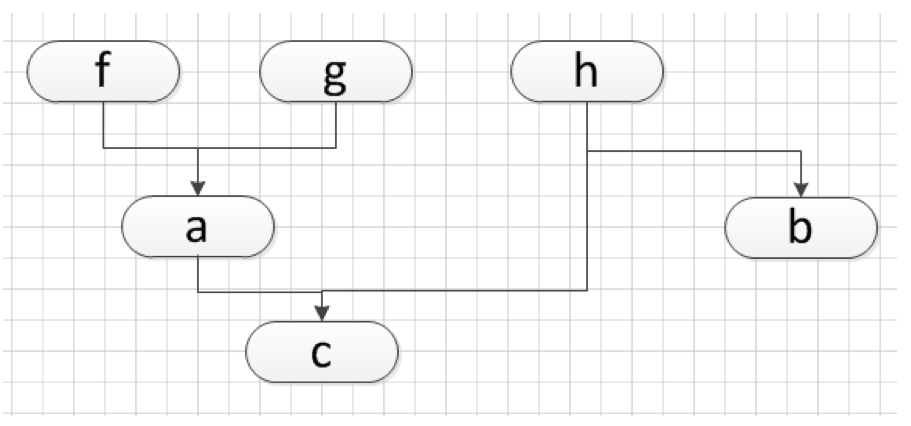
\includegraphics[scale=0.3]{flow.png}
\end{center}

We should only include formulae that belongs to functions that are
actually used. For example, to prove $a$'s contract, we should only
include $f$ and $g$ translations, and we would ask equinox:
$$ \dtrans{f},\dtrans{g},\dtrans{a},\ctrans{f},\ctrans{g} \vdash
\ctrans{a}$$


\section{Correctness of the translation}
For the translation to be useful, $\trans{M} \vdash \ctrans{f \in c} $
should imply that $f \in c$.


\section{Higher-orderness}
\label{ho}
Our current translation only considers fully applied functions and
first-order functions. For example, so far, we cannot give any
contract to $map$ because it would involve quantifying over a
function, a thing that is not first-order.

There is a possible workaround, which involves the ``app'' function
defined in our first-order logic. Assume we have a function $f$ that
is not fully applied somewhere in a module. We create the term
$f\_ptr$ which relates to $f$ by the equations given in figure~\ref{ho-fig}

This way, we can emulate quantification over function by quantifying
on their $ptr$ counterpart.


\begin{figure*}
$$ \forall x_1,\dots,x_n.~\full{f}(x_1,\dots,x_n) = f~x_1~x_2~\dots~x_n$$
$$ \cf{f} \tot \forall x_1,\dots,x_n.~\cf{x_1} \land \dots \land \cf{x_n} \to \cf{\full{f}(x_1,\dots,x_n)}$$
$$\forall g,x.~\cf{f} \land \cf{x} \to \cf{g~x}$$
\caption{Encoding of higher-orderness}
\label{ho-fig}
\end{figure*}

\section{Experiments}
That's how we roll.

\begin{figure*}
\begin{center}
    \begin{tabular}{l|c|c|c|c|c}
      Problem & Equinox & Equinox (+ weak) & SPASS & Vampire & E \\
      \hline
      Add.hs & 0.25 & 0.08 & 0.04 & 0.12 & 0.05\\
      BinaryTree.hs & 0.45 & 0.2 & 0.04 & 0.01 & 0.04 \\
      Branch.hs & 0.27 & 0.40 & 0.04 & 0.01 & 0.03 \\
      Copy.hs & 0.86 & 0.09 & 0.03 & 0.01 & 184.3 \\
      Head.hs & 0.32 & 0.29 & 0.03 & 0.03 & 4.2 \\
      Implies.hs & 3.24 & 0.32 & 0.06 & 0.02 & 0.11 \\
      Map.hs & 2.47 & 0.14 & 0.92 & 1.02 & $>$300 \\
      Mult.hs & $>$300 & 0.41 & 0.05 & 0.22 & 11.71 \\
      Multgt.hs & $>$300 & 1.24 & 0.62 & 1.31 & $>$300 \\
      NatEq.hs & 203.12 & 0.33 & 0.02 & 0.03 & 0.343 \\
      Odd.hs & 0.42 & 1.17 & 0.06 & 0.03 & $>$300 \\
      Reverse.hs & 72.32 & 0.12 & 0.05 & 0.02 & 0.038 \\
      Simple.hs & 0.07 & 0.04 & 0.01 & 0.01 & 0.022 \\
      Test.hs & 7.76 & 2.86 & 0.08 & 0.05 & $>$300 \\
      Test2.hs & 5.63 & 0.09 & 0.07 & 0.01 & 1.02 \\
    \end{tabular}
\end{center}
\caption{Comparison (in seconds) with other theorem provers}
\label{comparison}
\end{figure*}

\end{document}
